%% LyX 2.1.1 created this file.  For more info, see http://www.lyx.org/.
%% Do not edit unless you really know what you are doing.
\documentclass[twoside,english]{article}
\usepackage[utf8]{luainputenc}
\usepackage[a4paper]{geometry}
\geometry{verbose,tmargin=3.5cm,bmargin=3cm,lmargin=3cm,rmargin=3cm}
\setlength{\parskip}{\medskipamount}
\setlength{\parindent}{0pt}
\usepackage{color}
\usepackage{array}
\usepackage{float}
\usepackage{url}
\usepackage{multirow}
\usepackage{graphicx}

\makeatletter

%%%%%%%%%%%%%%%%%%%%%%%%%%%%%% LyX specific LaTeX commands.
\providecommand{\LyX}{L\kern-.1667em\lower.25em\hbox{Y}\kern-.125emX\@}
%% Because html converters don't know tabularnewline
\providecommand{\tabularnewline}{\\}

%%%%%%%%%%%%%%%%%%%%%%%%%%%%%% Textclass specific LaTeX commands.
\newenvironment{lyxlist}[1]
{\begin{list}{}
{\settowidth{\labelwidth}{#1}
 \setlength{\leftmargin}{\labelwidth}
 \addtolength{\leftmargin}{\labelsep}
 \renewcommand{\makelabel}[1]{##1\hfil}}}
{\end{list}}

%%%%%%%%%%%%%%%%%%%%%%%%%%%%%% User specified LaTeX commands.
\usepackage{fancyhdr}
\usepackage{afterpage}
\usepackage{framed}
\usepackage{settings}
\usepackage{pdflscape}
\usepackage{lscape}
\usepackage{color}   %May be necessary if you want to color links
\usepackage{hyperref}

%Set up settings
\setcounter{secnumdepth}{4}
\usepackage{hyperref}
\hypersetup{
    linktoc=all,     %set to all if you want both sections and subsections linked
}
 \usepackage{algorithm}
 \usepackage{algorithmicx}
\usepackage{algpseudocode}
\usepackage{tikz}
\usetikzlibrary{positioning}
\usetikzlibrary{arrows}

\makeatother

\usepackage{babel}
\begin{document}
\pagestyle{empty}

\begin{titlepage}

\begin{center}
\Large{\textsc{Politecnico di Milano}}\\
\Large{Scuola di Ingegneria Industriale e dell'Informazione}\\
\large{M.Sc. in Computer Science and Engineering}\\
\large{Dipartimento di Elettronica, Informazione e Bioingegneria}
\par\end{center}

\vspace{0.3cm}


\begin{center}
\begin{figure}[h]
\centering{}
\includegraphics[width=0.4\textwidth]{title-page/logo}
\end{figure}
\vspace{0.4cm}

\par\end{center}

\begin{center}
\huge{\textbf{myTaxiService}}\\
\vspace{0.2cm}

\par\end{center}

\begin{center}
\Large{Software Engineering 2 - Project}
\par\end{center}

\begin{center}
\vspace{0.9cm}
\Huge{\textbf{RASD}}\\
\Large{\textbf{Requirements Analysis and }\\
\textbf{Specification Document}}
\par\end{center}

\begin{center}
version 1.0
\par\end{center}

\begin{center}
6th November 2015
\par\end{center}

\begin{flushleft}
\vspace{0.5cm}

\par\end{flushleft}

\begin{flushright}
\begin{tabular}{ll}
Authors: & \tabularnewline
Alberto Maria METELLI & Matr. 850141\tabularnewline
Riccardo MOLOGNI & Matr. 852416\tabularnewline
\end{tabular}
\par\end{flushright}

\begin{flushleft}
\vspace{1.8cm}

\par\end{flushleft}

\begin{center}
{\large{}Academic Year 2015–2016}
\par\end{center}{\large \par}

\end{titlepage}


\clearpage{}

\afterpage{\null\newpage}

\clearpage{}

\pagestyle{fancy}
\fancypagestyle{plain}
\fancyhf{}
\fancyfoot{}
\fancyhead[LE,RO]{\thepage} 
\fancyhead[LO]{\slshape \rightmark} 
\fancyhead[RE]{\slshape \leftmark} 

\thispagestyle{empty}
\pagenumbering{roman}\tableofcontents{}\listoffigures


\clearpage{}

\afterpage{\null\newpage}

\clearpage{}

\pagenumbering{arabic}

\thispagestyle{empty}


\section{Introduction}


\subsection{Purpose}

The purpose of the RASD \emph{(Requirements Analysis and Specification
Document}) is to give a detailed description, analysis and specification
of the requirements for the \emph{myTaxiService} software. This document
will explain the \emph{goals} coming from stakeholders' expectations,
the characteristics of the application domain and the \emph{assumptions}
made to solve ambiguity and incompleteness. Starting from goals and
domain properties, \emph{requirements} will be formulated according
to a specific systematic methodology and then specified using both
informal and formal notations. However this document should not be
considered the final draft for the software specifications since in
the following phases several fixing may be necessary. 

The main objective of the RASD is to achieve good understanding among
\emph{analysts, developers, testers} and \emph{customers}, in particular
explaining both the application domain and the system to-be; it is
also aimed to be a solid base for project planning, software evaluation
and possible future maintenance activities. Therefore this document
is primarily intended to be proposed to the stakeholders for their
approval, to the analysts and programmers for the development of the
project and to the testing team the validation of the first version
of the software.


\subsection{Present system}

At the moment taxi service is entirely managed by phone calls. A passenger
who wants to request or reserve a taxi has to contact the call center.
In case of request, the call center operator moves the call to the
first available taxi, otherwise, in case of reservation, a taxi is
booked for the specific date, time and address provided by the passenger.
No available taxi queues management is implemented at the moment. 


\subsection{Scope}

The \emph{myTaxyService} is an application intended to optimize taxi
service in a large city, making the access to service simpler for
the passengers and ensuring a fair management of the taxi queues. 

Passengers will be able to request a taxi either through a web application
or a mobile app; of course the ``traditional'' ways to call for
a taxi, like a phone call or stopping the taxi along the road, will
be still available and integrated into the system to-be. The software
will make the procedure of calling a taxi simpler (by using GPS information
passenger doesn't need to know the address if the taxi is needed for
the current position) and more usable (passenger will be provided
with information about the waiting time). Moreover, by means of the
application, the passenger can reserve a taxi for a certain date and
time, specifying the origin and the destination of the ride.

Taxi drivers will use a mobile app to inform the system about their
availability and to confirm that they are going to take care of a
call (or to reject it for any reason). The software will make the
taxi management more efficient: the system will be able to identify
the position of each taxi by using GPS; the city will be divided in
virtual zones and a suitable distribution of the taxi among the zones
will automatically be computed.


\subsection{Definitions, acronyms, abbreviations }

In this paragraph all the terms, acronyms and abbreviations used in
the following sections are listed.


\subsubsection{Definitions}
\begin{itemize}
\item \emph{Request}: the action performed by the passenger of calling a
taxi for the current position.
\item \emph{Confirmed request}: a request that has been accepted by a taxi
driver.
\item \emph{Reservation}: the action performed by the passenger of booking
a taxi for a specific address and specific date and time.
\item \emph{Waiting time}: an estimation of the time required to taxi driver
to get to passenger's position.
\item \emph{Taxi code}: a unique alphanumerical identifier of the taxi.
\item \emph{Available taxi queues}: data structures used to store the references
of the available taxis, also used to select the taxis to which forward
a request.
\item \emph{Automatic geolocalization}: a system that provides the geographic
coordinates of the user. For this document it can be either a GPS
system or browser geolocalization.
\item \emph{Passengers' application}: the applications used by passengers
to access to TS system. For this document it can be either PMA or
PWA (see 1.4.2).
\item \emph{Login credentials}: username and password.
\item \textit{Notification}: communication from TS to taxi driver to move
to a specific zone.
\end{itemize}

\subsubsection{Acronyms}
\begin{itemize}
\item TS: myTaxiService.
\item PMA: Passenger mobile application.
\item PWA: Passenger web application.
\item TMA: Taxi driver mobile application.
\item QMS: Queue management system.
\end{itemize}

\subsubsection{Abbreviations}
\begin{itemize}
\item {[}Gn{]} n-th goal.
\item {[}Dn{]} n-th domain assumption.
\item {[}Rn.m{]} m-th requirement related to goal {[}Gn{]}.
\end{itemize}

\subsection{Actors}

In this paragraph a brief description of the various actors affected
by myTaxiService system is provided.
\begin{itemize}
\item \emph{Passenger}: a person that interacts with myTaxiService to request
or reserve a taxi. The interaction with the system may occur by means
of either PMA (mobile passenger) or PWA (web passenger). Each passenger
can be either a registered passenger or an unregistered passenger.
\item \emph{Registered passenger}: specific case of passenger that has already
registered to the system. He/She can login, request, reserve a taxi
and also visualize and modify the previous reservations.
\item \emph{Unregistered passenger}: specific case of passenger that hasn't
registered to the system. He/She can only request a taxi.
\item \emph{Taxi driver}: a person that drives a taxi and is associated
with myTaxiService. He/She interacts with the system confirming or
rejecting requests and informing the system about his/her availability
by means of TMA.
\item \emph{Call center operator}: a person working at the call center that
interacts with the system inserting taxi requests coming from phone
calls. 
\end{itemize}

\subsection{Requirement engineering approach}

In order to ensure a sound and complete requirement engineering activity,
we decided to follow a systematic technique for requirements formulation
proposed by Jackson and Zave. This approach is based on the distinction
between the \emph{machine}, the portion of the system to be developed
(myTaxiService in our case), and the \emph{world}, the portion of
the real world interacting with the machine. Machine and world are
tipically non disjoint, some phenomena may affect both of them, they
are known as shared phenomena. From this viewpoint, requirement engineering
consists in identifying phenomena shared between world and machine,
according to a set of \textbf{goals }(which express the desired behavior
of world phenomena, shared or not) and a set of \textbf{domain assumptions}
(assertions supposed to be always valid in the world). Formally a
set of \textbf{requirements }is complete if together with domain assumption
it ensures the goals.


\subsubsection{Goals}

Starting from the available documentation, integrated with some interviews
with the stakeholders, the following minimal goals has been identified.
\begin{lyxlist}{00.00.0000}
\item [{{[}G1{]}}] Allow a passenger to request a taxi for its current
position without registration.
\item [{{[}G2{]}}] Allow the passenger to visualize the waiting time and
the code of the incoming taxi for confirmed requests.
\item [{{[}G3{]}}] Allow a registered passenger to have a personal area.
\item [{{[}G4{]}}] Allow a registered passenger to reserve a taxi.
\item [{{[}G5{]}}] Allow a registered passenger to cancel or modify a previous
reservation. 
\item [{{[}G6{]}}] Allow a taxi driver to either accept or reject a request
coming from the system.
\item [{{[}G7{]}}] Allow a taxi driver to inform the system about his/her
availability.
\item [{{[}G8{]}}] Ensure that available taxi queues enjoy the properties
specified in sub paragraph 1.6.2.
\end{lyxlist}

\subsubsection{Queue management}

This paragraph is aimed to give a more precise definition of ``fair
management'' of the available taxi queues.

The city is divided into several zones, to each zone a taxi queue
is assigned. Each zone is characterized by a different load of requests
$n_{i}$ measured in request/minute. Let $N$ be the total number
of taxis available at a certain moment, the number $q_{i}$ of taxis
available in the zone $i$ has to be proportional to $n_{i}$, in
particular $q_{i}=Nn_{i}/\sum_{i}n_{i}$. Every time one taxi turns
from available to busy or out of service or viceversa a new distribution
of the taxis has to be computed; the taxis to be moved have to minimize
the cost of movement calculated as number of zones passed through.
To prevent too many movements, a fluctuation between -30\% and 30\%
from the value $q_{i}$ is accepted without performing taxi movements.


\subsection{Reference documents }
\begin{lyxlist}{00.00.0000}
\item [{{[}1{]}}] IEEE Software Engineering Standards Committee, “IEEE
Std 830-1998, IEEE Recommended Practice for Software Requirements
Specifications”, October 20, 1998. 
\item [{{[}2{]}}] P, Zave, M. Jackson, Four dark corners of requirements
engineering, TOSEM 1997.
\item [{{[}3{]}}] Software Abstractions: Logic, Language, and Analysis,
revised edition Edition by Daniel Jackson, MIT Press.
\item [{{[}4{]}}] Software Engineering 2 course slides.
\end{lyxlist}

\subsection{Overview}

This document is drawn up in accordance to the IEEE Std 830-1998 for
Software Requirements Specifications and it is composed of four sections
and an appendix.
\begin{itemize}
\item The first, this one, section gives a general description of the document
and brief information about the actors and the purposes of the software.
\item The second section provides an overview of the software, highlighting
the interaction with external system interfaces and explaining the
main functions carried out. It also focuses on constraints and domain
assumptions.
\item The third section is entirely dedicated to the derivation and specification
of the requirements. Several scenarios expressed in natural language
will be provided. A generalization of the set of scenarios will be
specified as a set of use cases that will be expressed both in natural
language and using UML use case diagram. For some groups of use cases
a dynamical description will be provided mainly using UML sequence
diagram. A high level conceptual description of the classes affected
by the system will be given using UML class diagram. For some of the
objects involved, we will design a UML state chart diagram showing
the evolution of its state. 
\item The fourth section presents a formalization of a subset of the requirements
using Alloy; some significant instances will be shown.
\item The appendix contains an interesting model of the goals, a brief description
of the tools used to produce this documents and the number of hours
each group member has worked towards the fulfillment of this deadline.\end{itemize}



\clearpage{}


\section{Function points}


\subsection{Introduction to cost estimation}

Estimating the cost of a software project is a non trivial task. Many
aspects contribute to determine the effort put in a software project
and relationships among the characteristics of the project team (number
of people, type of organization, ...), the features of the project
itself (complexity) and the environmental influences are typically
intricate and difficult to be estimated with an acceptable degree
of approximation. Therefore often we rely on the \emph{experience-based
techniques} where the estimation is made by an experienced manager
on the basis on the past projects and the application domain, sometimes
this task is performed by a team of experts (community-based estimation).
If no experts are available, or the domain of the application in too
specific only \emph{algorithmic cost modeling }is allowed. Those techniques
are based on a formulated approach to compute the project effort based
on estimates of product attributes. We will adopt the \emph{Function
Points} technique that was proposed by Allan Albrecht at IBM in 1965
and then COCOMOII that was developed around '80 based on the statistical
analysis performed by Barry Boehn on the basis on many real projects
coming from various domains.


\subsection{Function points approach}

There is an underlying hypothesis behind function points: the dimension
of software can be characterized by \emph{abstraction}. Therefore
after the architectural design (early in the project life cycle),
when the product model is almost clear, a rough evaluation of the
size of the software can be performed. Albrecht’s method identifies
and counts the number of function types within the software (actually
its model), those types constitutes the “external representation”
of an application, that is, its functionality as defined from an abstract
point of view. The types of functionalists are the following:
\begin{itemize}
\item \emph{Internal Logical File} (ILF): homogeneous set of data used and
managed by the application.
\item \emph{External Interface File} (EIF): homogeneous set of data used
by the application but generated and maintained by other applications.
\item \emph{External Input}: elementary operation to elaborate data coming
form the external environment.
\item \emph{External Output:} elementary operation that generates data for
the external environment; it usually includes the elaboration of data
from logic files.
\item \emph{External Inquiry}: elementary operation that involves input
and output, without significant elaboration of data from logic files.
\end{itemize}
The measure of the size of the software is given by the weighed average
of the function points (number of each function type listed above),
according to the following predefined table.\bigskip{}


\begin{center}
\begin{tabular}{>{\raggedright}p{5cm}|>{\centering}p{2cm}|>{\centering}p{2.5cm}|>{\centering}p{2cm}}
\hline 
\multirow{2}{5cm}{\textbf{Function type}} & \multicolumn{3}{>{\centering}p{7cm}}{\textbf{Weight}}\tabularnewline
\cline{2-4} 
 & \emph{Simple} & \emph{Average} & \emph{Complex}\tabularnewline
\hline 
\emph{EI (External Inputs)} & 3 & 4 & 6\tabularnewline
\hline 
\emph{EO (External Outputs)} & 4 & 5 & 7\tabularnewline
\hline 
\emph{EQ (External Inquiries)} & 3 & 4 & 6\tabularnewline
\hline 
\emph{ILF (Internal Logical Files)} & 7 & 10 & 15\tabularnewline
\hline 
\emph{ELF (External Logical Files)} & 5 & 7 & 10\tabularnewline
\hline 
\end{tabular}
\par\end{center}

\bigskip{}


The resulting sum is called UFP (Unadjusted Function Points). This
value can be further manipulated with the ``adjustment'' formula
to get an estimation of the effort, however the result is usually
little significant, therefore it is suggested to use the UFP in combination
with other effort estimation algorithms like COCOMO II. 


\subsection{Function point count}

In this section we present the function point count; for each type
of functionality we list the ones we have identified within the myTaxiService
system with the corresponding complexity and a rational for our choice.
According to the Albrecht definition, this process is performed by
abstraction therefore the main resource is the RASD in particular
the high level class diagram for the logical files and the use cases
for the inputs, outputs and inquiries.


\subsubsection{ILF (Internal logical files)}

The application includes a number of ILFs that will be used to store
information about:
\begin{itemize}
\item \emph{passengers}, in particular username, password, lastname, firstname,
email and address;
\item \emph{taxi drivers}, in particular username, password, firstname and
lastname;
\item \emph{taxis}, in particular the plate number, the code, the number
of seats and the current state;
\item \emph{requests}, in particular the date and time in which the request
is sent, the number of passengers, the location (geographical coordinates
and the address) of the passenger, possibly the waiting time and the
taxis assigned to the request itself;
\item \emph{reservations}, in particular the date and time in which the
request is sent, the number of passengers, the location (geographical
coordinates and the address) of both origin and destination and the
corresponding attached request;
\item \emph{zones}, in particular the name of the zone, the estimation of
the requests per minute and the adjacency relation among zones;
\item \emph{queues}: in particular the proper size of the queue (and also
the minimum and maximum number of taxis allowed) and the taxis belonging
to the queue with the corresponding position.
\end{itemize}
Each of these entities has a simple structure with a limited number
of fields except for the queue which requires a quite articulated
structure to manage positions and sizes of queues. Thus, we select
medium complexity for the latter and simple for the other ones. 

\[
ILF=6\cdot7+1\cdot10=52FPs
\]



\subsubsection{ELF (External logical files)}

myTaxiService has to interact with external systems, in particular
with the GPS and the GoogleMaps API therefore we can identify the
following ELFs:
\begin{itemize}
\item \emph{Address validation }requires the interaction with the GoogleMaps
API in order to check whether a string typed by the user corresponds
to a valid address.
\item \emph{Coordinate/Address translation} requires the interaction with
the GoogleMaps API in order to convert a coordinate retrieved by the
GPS into an address and viceversa.
\item \emph{Travelling time }requires the interaction with the GoogleMaps
API in order to compute the waiting time.
\item \emph{Passenger's geographic coordinates} requires the interaction
with the GPS system installed on the passenger smartphone or with
the browser geolocalization to retrieve the passenger's position.
\item \emph{Taxi geographic coordinates} requires the interaction with the
GPS installed on each taxi in order to find the position of the taxi
itself.
\end{itemize}
All those data items are very compact and they share the same simple
structure, so a simple complexity should be appropriate. 

\[
ELF=5\cdot5=25FPs
\]



\subsubsection{EI (External inputs)}

Since myTaxiService is an application characterized of having a high
degree of interaction with the final user, we can identify the following
EI.
\begin{itemize}
\item \emph{Registration}: this function requires the exchange of a relevant
amount of information (username, password, lastname, firstname, email
and address), in addition some checks has to be performed (like check
that the username is not already used), so we can consider medium
complexity with a contribution of 4 FPs.
\item \emph{Login/Logout}: this function is standard and requires exchange
of basic structured information and simple operations, so it can be
considered simple with a contribution of 3 FPs.
\item \emph{Request}: this function requires the insertion of some data
(like address), the interaction with external systems (like GPS and
GoogleMaps API) and with the DBMS, therefore it can be considered
complex with a contribution of 6 FPs.
\item \emph{Taxi selection}: this function requires non trivial elaborations
related to the algorithm used to select the taxis to fulfill a request/reservation;
it requires interaction with the DBMS and external systems therefore
it can be considered complex with a contribution of 6 FPs.
\item \emph{Taxi queue management}: this function requires the execution
of the algorithm described in the design document for the taxi movement,
in addition it requires to interact with external systems and the
DBMS therefore it can be considered complex with a contribution of
6 FPs.
\item \emph{Reservation}: this function requires interaction with the DBMS
and with external systems, it has also to instantiate a new request
associated to the reservation and to perform validity checks on the
inserted data, therefore it can be considered complex with a contribution
of 6 FPs.
\item \emph{Modify reservation}: this function can be considered an extension
of Reservation, adding a small new functionality, therefore it can
be considered simple with a contribution of 3 FPs.
\item \emph{Cancel reservation}: this function can be considered an extension
of Reservation, adding a small new functionality, therefore it can
be considered simple with a contribution of 3 FPs.
\item \emph{Request evaluation}: this function requires to interact with
the TMA and the analysis of the taxi queues, so it can be considered
medium complexity with a contribution of 4 FPs.
\item \emph{Inform about availability}: this function requires to check
some conditions to validate the state changing of the taxi driver,
it can be considered medium complexity with a contribution of 4 FPs.
\item \emph{Insert phone request}: this function is just reduced to Request
therefore it can be considered simple with a contribution of 3 FPs.
\end{itemize}
\[
EI=4\cdot3+3\cdot4+4\cdot6=48FPs
\]



\subsubsection{EO External output}

The only external outputs generated by the myTaxiService are:
\begin{itemize}
\item \emph{Movement notification: }that function is performed by the system
to communicate to the taxi driver the notification of the movement,
since it requires the evaluation of the taxi queues it can be considered
medium complexity with a contribution of 5 FPs.
\item \emph{Request notification: }this function is performed in order to
communicate to the taxi driver a request to be carried out, it requires
only to send information about the address of the passenger therefore
it can be considered simple with a contribution of 4 FPs.
\end{itemize}
\[
EI=1\cdot4+1\cdot5=9FPs
\]



\subsubsection{EQ External inquiries}

We identified the following EQs.
\begin{itemize}
\item \emph{Visualize request info}: this function allows passenger, both
registered or not, to visualize the information about the last request
including waiting time and the number of incoming taxi.
\item \emph{Visualize previous reservations}: this function allows registered
passengers to visualize the previous sent reservations.
\item \emph{Visualize previous requests (taxi driver)}: this function allows
the taxi driver to visualize the previous requests carried out.
\end{itemize}
All these functions requires the interaction with the DBMS therefore
they can be considered medium complexity.

\[
EI=3\cdot4=12FPs
\]



\subsubsection{UFP Unadjusted Function Points count}

Here we summarize the number of function points identified in every
category and we provide the UFP (Unadjusted Function Points count)
which could possibly be adjusted to take into account organizational
aspects and get an estimation of the effort, however this approach
is typically very imprecise therefore we will use UFP in combination
with the COCOMO approach.

\bigskip{}


\noindent \begin{center}
\begin{tabular}{>{\raggedright}p{5cm}|>{\centering}p{1.5cm}}
\hline 
\multicolumn{1}{l|}{\textbf{Function type}} & \textbf{FPs}\tabularnewline
\hline 
\hline 
\emph{ILF (Internal Logical Files)} & 52\tabularnewline
\hline 
\emph{ELF (External Logical Files)} & 25\tabularnewline
\hline 
\emph{EI (External Inputs)} & 48\tabularnewline
\hline 
\emph{EO (External Outputs)} & 9\tabularnewline
\hline 
\emph{EQ (External Inquiries)} & 12\tabularnewline
\hline 
\end{tabular}
\par\end{center}

\bigskip{}


Thus, we get at the end the value of UFP

\textbf{
\[
UFP=ILF+ELF+EI+EO+EQ=146FPs
\]
}

Here we provide an histogram representing the number of function points
for each category.

\begin{figure}[H]
\noindent \begin{centering}
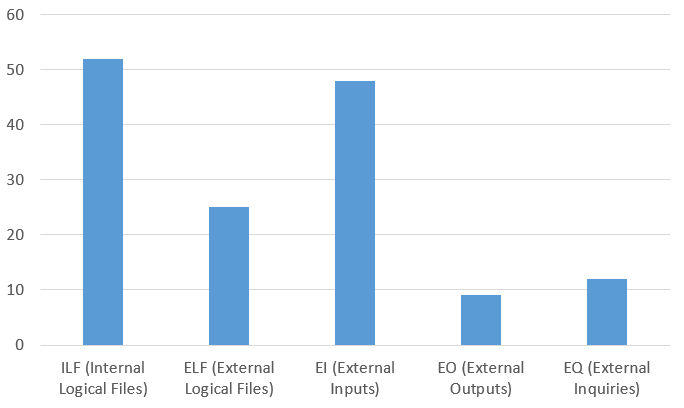
\includegraphics[scale=0.7]{function-points/fp}
\par\end{centering}

\protect\caption{Function Points Histogram}
\end{figure}



\subsection{Lines of code count}

The Unadjusted Function Points (UFP) can be used to provide an estimation
of the number of lines of code (SLOC) of the final project according
to the specific implementation language chosen. Instead of referring
to the ``traditional'' table proposed by Jones 1996 for the conversion
factor, which by the way does not include a value for JEE, we adopt
the more recent Function Points Language Table proposed in {[}7{]}.
myTaxiService is intended to be implemented with JEE, the table provides
a range for the conversion factor SLOC/FP

\bigskip{}


\noindent \begin{center}
\begin{tabular}{>{\centering}p{2cm}|>{\centering}p{2cm}|>{\centering}p{2cm}|>{\centering}p{2cm}|>{\centering}p{2cm}}
\hline 
\textbf{Language} & \emph{Average} & \emph{Median} & \emph{Low} & \emph{High}\tabularnewline
\hline 
J2EE & 46 & 49 & 15 & 67\tabularnewline
\hline 
\end{tabular}
\par\end{center}

\bigskip{}


Not having precise information about the complexity of the implementation
we think an average value should be proper, so $SLOC/FP=46$ and we
get the value of SLOC.

\[
SLOC=SLOC/FP\cdot UFP=46\cdot146=6716
\]


Notice that this value does not capture, for the most part, the client
side of the application and the web server. Since both PMA, TMA and
web server do not perform meaningful functions at requirement level
but just auxiliary functions they are not highlighted in the function
points count, however from an implementation point of view they might
require a relevant effort.


\clearpage{}


\section{COCOMO II}

In this section, after a brief introduction to COCOMO II, we present
the application of the method to myTaxiService system in order to
get the effort estimation and the expected duration of the project.


\subsection{COCOMOII approach}

Mainly taken from {[}6{]}.

COCOMO II is an updated version of COCOMO 81 which is based on a linear
regression model of the function relating the size of the project
and the effort. However the original version was affected by old time
and non realistic assumptions on the \emph{software lifecycle}, in
particular it assumed that the development process followed the traditional
waterfall scheme, that requirements were supposed to be stable during
the project duration and that the documentation was written incrementally.
COCOMO II is able to overcome those limitation and provide a reasonable
estimation of both the effort and the duration of the project. In
the following subsection we will describe the model.


\subsubsection{Effort Equation}

In COCOMO II \emph{effort} is expressed as \emph{Person-Months} (PM).
\footnote{A person month is the amount of time one person spends working on
the software development project for one month. COCOMO II treats the
number of person-hours per person-month, PH/PM, as an adjustable factor
with a nominal value of 152 hours per Person-Month.%
}The \emph{Effort equation} allows to compute the effort as a function
of the \emph{size} of software development expressed in KSLOC (thousand
of SLOC)%
\footnote{The SLOC in COCOMO represent only the line of codes that are going
to be delivered and they have to be computed as \emph{logical} SLOC.%
} that can be obtained by the Function Points method, a constant, A,
an exponent, E, and a number of values called\emph{ effort multipliers}
(EM). The number of effort multipliers depends on the model. 

\[
Effort=PM=A\cdot Size^{E}\cdot\prod_{i=1}^{n}EM_{i}
\]


where $A=2.94$ for COCOMO II. We now present how to compute $E$
and each $EM_{i}$%
\footnote{Sometimes the overall contribution of the $EM_{i}$ is called $EAF$
(Effort Adjustment Factor) which is trivially defined as $EAF=\prod_{i=i}^{n}EM_{i}$.%
}.


\subsubsection{Software Scale Drivers}

The exponent E in the effort equation is an aggregation of five \emph{scale
factors} (SF, also referred to \emph{scale drivers} SD) is related
to economic, organizational and technical aspects of the environment
in which the project is going to be developed. In particular if account
for the relative economies or diseconomies of scale encountered for
software projects of different sizes {[}Banker et al. 1994{]}. %
\footnote{If E$<$1.0, the project exhibits economies of scale. If the product’s
size is doubled, the project effort is less than doubled. The project’s
productivity increases as the product size is increased. Some project
economies of scale can be achieved via project-specific tools (e.g.,
simulations, testbeds). For small projects, fixed start-up costs such
as tool tailoring and setup of standards and administrative reports
are often a source of economies of scale. If E$=$1.0, the economies
and diseconomies of scale are in balance. This linear model is often
used for cost estimation of small projects. If E$>$1.0, the project
exhibits diseconomies of scale.%
}

The value of E is a contribution of the following scale factors.
\begin{lyxlist}{00.00.0000}
\item [{PREC}] \emph{Precedentedness}: reflects the previous experience
of the organization with this type of project. Very low means no previous
experience, Extra high means that the organization is completely familiar
with this application domain.
\item [{FLEX}] \emph{Development Flexibility}: reflects the degree of flexibility
in the development process. Very low means a prescribed process is
used; Extra high means that the client only sets general goals.
\item [{RESL}] \emph{Architecture / Risk Resolution}: reflects the extent
of risk analysis carried out. Very low means little analysis, Extra
high means a complete a thorough risk analysis.
\item [{TEAM}] \emph{Team Cohesion}: reflects how well the development
team know each other and work together. Very low means very difficult
interactions, Extra high means an integrated and effective team with
no communication problems.
\item [{PMAT}] \emph{Process Maturity}: reflects the process maturity of
the organization. The computation of this value depends on the CMM
(Capability Maturity Model)%
\footnote{CMM is a development model created to represent the ``maturity''
of software development process as the degree of formality and optimization
of processes, from ad hoc practices, to formally defined steps, to
managed result metrics, to active optimization of the processes. Nowadays
the extension CMMI (Capability Maturity Model Integration) is used.%
} Questionnaire but an estimate can be achieved by subtracting the
CMM process maturity level from 5. 
\end{lyxlist}
The following table provides the rating levels for the COCOMO II scale
factors. The selection of scale factors is based on the rationale
that they are a significant source of exponential variation on a project’s
effort or productivity variation. Each scale factors has a range of
rating levels, from Very Low to Extra High and each rating level has
a weight.

\medskip{}


\noindent \begin{center}
\begin{tabular}{c|>{\centering}p{1.5cm}|>{\centering}p{1.5cm}|>{\centering}p{1.5cm}|>{\centering}p{1.5cm}|>{\centering}p{1.5cm}|>{\centering}p{1.5cm}}
\hline 
\emph{Scale Factor } & \emph{Very Low} & \emph{Low} & \emph{Nominal} & \emph{High} & \emph{Very High} & \emph{Extra High}\tabularnewline
\hline 
\hline 
PREC  & {\small{}thoroughly unprecedented}{\small \par}

\textbf{\small{}6.20} & {\small{}largely unprecedented}{\small \par}

\textbf{\small{}4.96} & {\small{}somewhat unprecedented}{\small \par}

\textbf{\small{}3.72} & {\small{}generally familiar}{\small \par}

\textbf{\small{}2.48} & {\small{}largely familiar}{\small \par}

\textbf{\small{}1.24} & {\small{}thoroughly familiar}{\small \par}

\textbf{\small{}0.00}\tabularnewline
\hline 
FLEX  & {\small{}rigorous}{\small \par}

\textbf{\small{}5.07} & {\small{}occasional relaxation}{\small \par}

\textbf{\small{}4.05} & {\small{}some relaxation}{\small \par}

\textbf{\small{}3.04} & {\small{}general conformity }{\small \par}

\textbf{\small{}2.03} & {\small{}some conformity }{\small \par}

\textbf{\small{}1.01} & {\small{}general goals}{\small \par}

\textbf{\small{}0.00}\tabularnewline
\hline 
RESL & {\small{}little (20\%)}{\small \par}

\textbf{\small{}7.07} & {\small{}some (40\%) }{\small \par}

\textbf{\small{}5.65} & {\small{}often (60\%) }{\small \par}

\textbf{\small{}4.24} & {\small{}generally (75\%) }{\small \par}

\textbf{\small{}2.83} & {\small{}mostly (90\%) }{\small \par}

\textbf{\small{}1.41} & {\small{}full (100\%)}{\small \par}

\textbf{\small{}0.00}\tabularnewline
\hline 
TEAM  & {\small{}very difficult interactions }{\small \par}

\textbf{\small{}5.48} & {\small{}some difficult interactions }{\small \par}

\textbf{\small{}4.38} & {\small{}basically cooperative }{\small \par}

\textbf{\small{}3.29} & {\small{}interactions largely cooperative }{\small \par}

\textbf{\small{}2.19} & {\small{}highly cooperative }{\small \par}

\textbf{\small{}1.10} & {\small{}seamless interactions }{\small \par}

\textbf{\small{}0.00}\tabularnewline
\hline 
PMAT  & {\small{}SW-CMM Level 1 Lower}{\small \par}

\textbf{\small{}7.80} & {\small{}SW-CMM Level 1 Upper }{\small \par}

\textbf{\small{}6.24} & {\small{}SW-CMM Level 2 }{\small \par}

\textbf{\small{}4.68} & {\small{}SW-CMM Level 3 }{\small \par}

\textbf{\small{}3.12} & {\small{}SW-CMM Level 4 }{\small \par}

\textbf{\small{}1.56} & {\small{}SW-CMM Level 5 }{\small \par}

\textbf{\small{}0.00}\tabularnewline
\hline 
\end{tabular}
\par\end{center}

\medskip{}


To have a complete description of the meaning of each scale factor,
please refer to {[}6{]} where also assessment methods are proposed. 

Once the value of each scale factor $SF_{j}$ is determined the value
of the exponent $E$ can be computed using the following formula.

\[
E=B+0.01\cdot\sum_{j=i}^{5}SF_{j}
\]


where $B=0.91$ for COCOMO II. Notice that if all scale factors are
judged as Nominal the resulting exponent value is $E=1.0997$.


\subsubsection{Software Cost Drivers}

\emph{Cost drivers} are used to capture characteristics of the software
development that affect the effort to complete the project. All COCOMO
II cost drivers have qualitative rating levels that express the impact
of the driver on development effort. These ratings can range from
Extra Low to Extra High. Each rating level of every multiplicative
cost driver has a value, called an \emph{effort multiplier} (EM),
associated with it. The EM value assigned to a multiplicative cost
driver's nominal rating is 1.00. All those are intended to be evaluated
in post-architecture/early-design phase and they are organized in
categories, for the complete description refer to {[}6{]}.
\begin{itemize}
\item \emph{Product} factors account for variation in the effort required
to develop software caused by characteristics of the product under
development. A product that is complex, has high reliability requirements,
or works with a large testing database will require more effort to
complete.

\begin{lyxlist}{00.00.0000}
\item [{RELY}] Required Software Reliability 
\item [{DATA}] Data Base Size 
\item [{CPLEX}] Product Complexity 
\item [{RUSE}] Developed for Reusability 
\item [{DOCU}] Documentation Match to Lifecycle Needs
\end{lyxlist}
\item \emph{Personnel} factors have the strongest influence in determining
the amount of effort required to develop a software product. The Personnel
Factors are for rating the development team’s capability and experience
– not the individual. These ratings are most likely to change during
the course of a project reflecting the gaining of experience or the
rotation of people onto and off the project. 

\begin{lyxlist}{00.00.0000}
\item [{ACAP}] Analyst Capability 
\item [{PCAP}] Programmer Capability 
\item [{PCON}] Personnel Continuity 
\item [{AEXP}] Application Experience 
\item [{PEXP}] Platform Experience 
\item [{LTEX}] Language and Toolset Experience 
\end{lyxlist}
\item \emph{Platform} factors refers to the target-machine complex of hardware
and infrastructure software (previously called the virtual machine).
The factors have been revised to reflect this as described in this
section. Some additional platform factors were considered, such as
distribution, parallelism, embeddedness, and real-time operations. 

\begin{lyxlist}{00.00.0000}
\item [{TIME}] Time Constraint 
\item [{STOR}] Storage constraint
\item [{PVOL}] Platform Volatility 
\end{lyxlist}
\item \emph{Project} factors account for influences on the estimated effort
such as use of modern software tools, location of the development
team, and compression of the project schedule. 

\begin{lyxlist}{00.00.0000}
\item [{TOOL}] Use of Software Tools 
\item [{SITE}] Multisite Development 
\item [{SCED}] Required Development Schedule 
\end{lyxlist}
\end{itemize}

\subsubsection{Schedule estimation }

The \emph{Schedule equation} allows to determine the \emph{Time to
Develop}, TDEV, expressed in number of months required to complete
the software project.

\[
Duration=TDEV=C\cdot(PM)^{(D+0.2(E-B))}
\]


where $C=3.67$, $D=0.28$, $B=0.91$.

C is a TDEV coefficient that can be calibrated, $PM$ is the estimated
effort, D is a TDEV scaling base exponent that can also be calibrated.
E is the effort scaling exponent derived as the sum of project scale
factors and B as the calibrated scale factor base-exponent. If we
also know the average monthly salary $S$ of the personnel we can
estimate the personnel cost.%
\footnote{Notice that this is very different from the overall cost of the project
since we do not take into account overheads (buildings, heating, lighting,
...).%
}

\[
Cost=PM\cdot S
\]



\subsubsection{Number of people estimation }

Using PM and TDEV calculated before we can give an estimation of the
number of required people.

\[
N=\frac{PM}{TDEV}
\]



\subsection{COCOMO II calculation}

In this subsection we perform the COCOMO II estimation starting from
the SLOC determined in the previous stage thanks to Function Points
approach. Given the academic context and the fact that implementation
was not performed we will try to both perform the calculation with
\begin{itemize}
\item all SFs and CDs rated as nominal and
\item SFs and CDs rated according our opinion with respect to a reasonable
implementation phase.
\end{itemize}
Then we compere the results obtained by the two different approaches.
We also assume that each person involved in the project is payed 2500\$
per month. To easily compute the PM and TDEV we refer to the online
tool \url{http://csse.usc.edu/tools/COCOMOII.php}.


\subsubsection{COCOMO II with all SFs and CDs nominal}

If we assume to set all SFs and CDs to nominal we get the parameters
$E=1.0997$ and $EAF=1$ therefore knowing that $Size=KSLOC=6.716$
we get the following results.

\[
Effort=PM=2.94\cdot(6.716)^{1.0997}\cdot1=23.9\;\mathrm{person-month}
\]


\[
Duration=TDEV=3.67\cdot(23.9)^{0.31794}=10.5\;\mathrm{months}
\]


\[
Cost=23.9\cdot2500\$=59684\;\mathrm{\$}
\]


\[
N=\frac{23.9}{10.5}=2.276\;\mathrm{person}
\]


We report some tables and graphs taken from the web site.

\textbf{Acquisition Phase Distribution}

\noindent \begin{center}
\begin{tabular}{>{\centering}p{2.5cm}||>{\centering}p{2.5cm}|>{\centering}p{2.5cm}|>{\centering}p{2.5cm}|>{\centering}p{2.5cm}}
\hline 
\textbf{Phase} & \emph{Effort (Person-months) } & \emph{Schedule (Months)} & \emph{Average Staff } & \emph{Cost (Dollars)}\tabularnewline
\hline 
\hline 
\textcolor{red}{Inception} & 1.4 & 1.3 & 1.1 & 3581\tabularnewline
\hline 
\textcolor{magenta}{Elaboration} & 5.7 & 3.9 & 1.5 & 14324\tabularnewline
\hline 
\textcolor{blue}{Construction} & 18.1 & 6.5 & 2.8 & 45360\tabularnewline
\hline 
\textcolor{green}{Transition} & 2.9 & 1.3 & 2.2 & 7162\tabularnewline
\hline 
\end{tabular}
\par\end{center}

\textbf{Software Effort Distribution for RUP/MBASE (Person-Months)}

\noindent \begin{center}
\begin{tabular}{c||>{\centering}p{2cm}|>{\centering}p{2cm}|>{\centering}p{2cm}|>{\centering}p{2cm}}
\hline 
\textbf{Phase/Activity} & Inception  & Elaboration  & Construction  & Transition\tabularnewline
\hline 
\hline 
\emph{Management} & 0.2 & 0.7 & 1.8 & 0.4\tabularnewline
\hline 
\emph{Environment/CM} & 0.1 & 0.5 & 0.9 & 0.1\tabularnewline
\hline 
\emph{Requirements} & 0.5 & 1.0 & 1.5 & 0.1\tabularnewline
\hline 
\emph{Design} & 0.3 & 2.1 & 2.9 & 0.1\tabularnewline
\hline 
\emph{Implementation} & 0.1 & 0.7 & 6.2 & 0.5\tabularnewline
\hline 
\emph{Assessment} & 0.1 & 0.6 & 4.4 & 0.7\tabularnewline
\hline 
\emph{Deployment} & 0.0 & 0.2 & 0.5 & 0.6\tabularnewline
\hline 
\end{tabular}
\par\end{center}

\textbf{Staffing profile}

\noindent \begin{center}
\begin{figure}[H]
\noindent \begin{centering}
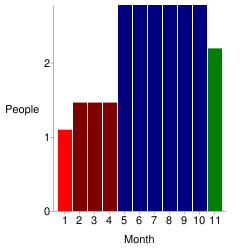
\includegraphics{COCOMOII/images/allnominal}
\par\end{centering}

\protect\caption{COCOMO II histogram - all nominal}
\end{figure}

\par\end{center}

From now on we will discuss how to rate Scale Drivers and Cost Drivers
for myTaxiService.


\subsubsection{Software Scale Drivers}

In the following table we describe for each scale driver the motivations
behind the rating level choice, we refer to the descriptors stated
in {[}6{]}.

\noindent \begin{center}
\begin{tabular}{c|>{\raggedright}p{8.5cm}|>{\centering}p{1.5cm}|>{\centering}p{1.5cm}}
\hline 
\emph{Scale Factor} & \emph{Motivation} & \emph{Rating level} & \emph{Weight}\tabularnewline
\hline 
\hline 
PREC  & \begin{itemize}
\item {\small{}Organizational understanding of product objectives: Thorough}{\small \par}
\item {\small{}Experience in working with related software systems: Moderate}{\small \par}
\item {\small{}Concurrent development of associated new hardware and operational
procedures: Moderate}{\small \par}
\item {\small{}Need for innovative data processing architectures, algorithms:
Some}\end{itemize}
 & Nominal & 3.72\tabularnewline
\hline 
FLEX  & \begin{itemize}
\item {\small{}Need for software conformance with preestablished requirements:
Basic (many aspects were not clearly specified)}{\small \par}
\item {\small{}Need for software conformance with external interface specifications:
Considerable (integration with some external systems needed)}{\small \par}
\item {\small{}Combination of inflexibilities above with premium on early
completion: High}\end{itemize}
 & High & 2.03\tabularnewline
\hline 
RESL & \begin{itemize}
\item {\small{}Percent of development schedule devoted to establishing architecture,
given general product objectives: 25}{\small \par}
\item {\small{}Percent of required top software architects available to
project: 80}{\small \par}
\item {\small{}Tool support available for resolving risk items, developing
and verifying architectural specs: Some}{\small \par}
\item {\small{}Level of uncertainty in key architecture drivers: mission,
user interface, COTS, hardware, technology, performance: Considerable}{\small \par}
\item {\small{}Number and criticality of risk items: Some}\end{itemize}
 & High & 2.83\tabularnewline
\hline 
\end{tabular}
\par\end{center}

\noindent \begin{center}
\begin{tabular}{c|>{\raggedright}p{8.5cm}|>{\centering}p{1.5cm}|>{\centering}p{1.5cm}}
\hline 
\emph{Scale Factor} & \emph{Motivation} & \emph{Rating level} & \emph{Weight}\tabularnewline
\hline 
\hline 
TEAM  & \begin{itemize}
\item {\small{}Consistency of stakeholder objectives and cultures: Strong}{\small \par}
\item {\small{}Ability, willingness of stakeholders to accommodate other
stakeholders’ objectives: Considerable}{\small \par}
\item {\small{}Experience of stakeholders in operating as a team: Considerable}{\small \par}
\item {\small{}Stakeholder teambuilding to achieve shared vision and commitments:
Considerable}\end{itemize}
 & Very High & 1.10\tabularnewline
\hline 
PMAT  & {\small{}Answering to the KPAs (Key Process Area) we get a value of
$KPA%=\ensuremath{30}
$ thus the corresponding EPML (Equivalent Processing Maturity Level)
is 1.5} & Nominal & 4.68\tabularnewline
\hline 
\end{tabular}
\par\end{center}

We obtain a total value for the exponent E of 

\[
E=B+0.01\cdot\sum_{j=i}^{5}SF_{j}=1.0536
\]


Notice that the value of the exponent is smaller with respect to the
one obtained setting all SFs to nominal, this means that we are benefiting
of the quality of the environment in which the software is developed.

\newpage{}


\subsubsection{Software Cost Drivers}

In the following table we describe for each cost driver the motivations
behind the rating level choice, we refer to the descriptors stated
in {[}6{]}. Whenever the information for selecting the most appropriate
rating level is not available we adopt nominal value.

\noindent \begin{center}
\begin{tabular}{c|>{\raggedright}p{8cm}|>{\centering}p{1.5cm}|>{\centering}p{1.5cm}}
\hline 
\emph{Cost Driver } & \emph{Motivation} & \emph{Rating level} & \emph{Effort multiplier}\tabularnewline
\hline 
\hline 
RELY & {\small{}Moderate, easily recoverable losses.} & Nominal & 1.00\tabularnewline
\hline 
DATA & {\small{}10 $\leq$Testing DB bytes/Pgm SLOC$<$100} & Nominal & 1.00\tabularnewline
\hline 
CPLEX & \begin{itemize}
\item \emph{\small{}Control Operations}{\small{}: Highly nested structured
programming operators with many compound predicates. Queue and stack
control. Homogeneous, distributed processing. Single processor soft
real-time control. }{\small \par}
\item \emph{\small{}Computational Operations:}{\small{} Use of standard
math and statistical routines. Basic matrix/vector operations. }{\small \par}
\item \emph{\small{}Device dependent Operations}{\small{}: Operations at
physical I/O level (physical storage address translations; seeks,
reads, etc.). Optimized I/O overlap. }{\small \par}
\item \emph{\small{}Data Management Operations}{\small{}: Multi-file input
and single file output. Simple structural changes, simple edits. Complex
COTS-DB queries, updates. }{\small \par}
\item \emph{\small{}User Interface Management Operations}{\small{}: Simple
use of widget set. }\end{itemize}
 & High & 1.17\tabularnewline
\hline 
RUSE & {\small{}Across program}%
\footnote{“Across project” could apply to reuse across the modules in a single
financial applications project. “Across program” could apply to reuse
across multiple financial applications projects for a single organization.
“Across product line” could apply if the reuse is extended across
multiple organizations. “Across multiple product lines” could apply
to reuse across financial, sales, and marketing product lines.%
} & High & 1.07\tabularnewline
\hline 
DOCU & {\small{}Right-sized to life-cycle needs } & Nominal & 1.00\tabularnewline
\hline 
ACAP & {\small{}Analysts in the 75th percentile} & High & 0.85\tabularnewline
\hline 
PCAP & {\small{}Programmes in the 75th percentile} & High & 0.88\tabularnewline
\hline 
PCON & {\small{}Personell turnover 3\% / year } & Very High & 0.81\tabularnewline
\hline 
AEXP & {\small{}≤ 2 months } & Very Low & 1.22\tabularnewline
\hline 
PEXP & {\small{}≤ 2 months } & Very Low & 1.19\tabularnewline
\hline 
LTEX & {\small{}1 year} & Nominal & 1.00\tabularnewline
\hline 
TIME & {\small{}85\% use of available execution time} & Very High & 1.29\tabularnewline
\hline 
STOR & {\small{}≤ 50\% use of available storage} & Nominal & 1.00\tabularnewline
\hline 
PVOL & {\small{}Major change every 12 mo.; Minor change every 1 mo. } & Low & 0.87\tabularnewline
\hline 
TOOL & {\small{}basic lifecycle tools, moderately integrated } & Nominal & 1.00\tabularnewline
\hline 
SITE & \begin{itemize}
\item \emph{\small{}Collocation Descriptors}{\small{}: Same city or metro.
area }{\small \par}
\item \emph{\small{}Communications Descriptors}{\small{}: Wideband electronic
communication. }\end{itemize}
 & High & 0.93\tabularnewline
\hline 
SCED & {\small{}Shedule compression 130\% of nominal } & High & 1.00\tabularnewline
\hline 
\end{tabular}
\par\end{center}

We obtain a total value for the EAF of

\[
EAF=\prod_{i=i}^{n}EM_{i}=1.149
\]


Note that the value of EAF is grater than the one obtained assuming
all CDs as nominal, this mean that CDs turn out to affect negatively
the overall effort.


\subsubsection{Effort estimation and schedule estimation}

Considering the values computed above, $E=1.0536$ and $EAF=1.149$,
and knowing that $Size=KSLOC=6.716$ we get the following results.

\[
Effort=PM=2.94\cdot(6.716)^{1.0536}\cdot1.149=25.1\;\mathrm{person-month}
\]


\[
Duration=TDEV=3.67\cdot(25.1)^{0.30872}=13.8\;\mathrm{months}
\]


\[
Cost=25.1\cdot2500\$=62832\;\mathrm{\$}
\]


\[
N=\frac{25.1}{13.8}=1.82\;\mathrm{person}
\]


Note that this second result is just slightly different with respect
to the one obtained with all nominal SFs and CDs, in fact the effort
here is grater of 1.2 person-month and also the duration is increased
of 3.3 months; however the required number of people is still around
2. 

We report some tables and graphs taken from the web site.

\textbf{Acquisition Phase Distribution}

\noindent \begin{center}
\begin{tabular}{>{\centering}p{2.5cm}||>{\centering}p{2.5cm}|>{\centering}p{2.5cm}|>{\centering}p{2.5cm}|>{\centering}p{2.5cm}}
\hline 
\textbf{Phase} & \emph{Effort (Person-months) } & \emph{Schedule (Months)} & \emph{Average Staff } & \emph{Cost (Dollars)}\tabularnewline
\hline 
\hline 
\textcolor{red}{Inception} & 1.5 & 1.7 & 0.9 & 3770\tabularnewline
\hline 
\textcolor{magenta}{Elaboration} & 6.0 & 52. & 1.2 & 15080\tabularnewline
\hline 
\textcolor{blue}{Construction} & 19.1 & 8.6 & 2.2 & 47753\tabularnewline
\hline 
\textcolor{green}{Transition} & 3.0 & 1.7 & 1.7 & 7540\tabularnewline
\hline 
\end{tabular}
\par\end{center}

\textbf{Software Effort Distribution for RUP/MBASE (Person-Months)}

\noindent \begin{center}
\begin{tabular}{c||>{\centering}p{2cm}|>{\centering}p{2cm}|>{\centering}p{2cm}|>{\centering}p{2cm}}
\hline 
\textbf{Phase/Activity} & Inception  & Elaboration  & Construction  & Transition\tabularnewline
\hline 
\hline 
\emph{Management} & 0.2 & 0.7 & 1.9 & 0.4\tabularnewline
\hline 
\emph{Environment/CM} & 0.2 & 0.5 & 1.0 & 0.2\tabularnewline
\hline 
\emph{Requirements} & 0.6 & 1.1 & 1.5 & 0.1\tabularnewline
\hline 
\emph{Design} & 0.3 & 2.2 & 3.1 & 0.1\tabularnewline
\hline 
\emph{Implementation} & 0.1 & 0.8 & 6.5 & 0.6\tabularnewline
\hline 
\emph{Assessment} & 0.1 & 0.6 & 4.6 & 0.7\tabularnewline
\hline 
\emph{Deployment} & 0.0 & 0.2 & 0.6 & 0.6\tabularnewline
\hline 
\end{tabular}
\par\end{center}

\textbf{Staffing profile}

\noindent \begin{center}
\begin{figure}[H]
\noindent \begin{centering}
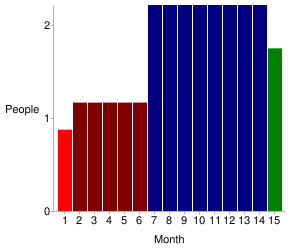
\includegraphics{COCOMOII/images/real}
\par\end{centering}

\protect\caption{COCOMO II histogram}
\end{figure}

\par\end{center}


\clearpage{}


\section{Tasks and schedule}

\emph{Project planning} is typically a in iterative process that starts
at project initiation and continues evolving. In order to set up a
suitable \emph{project schedule}, and in particular decide the time
and resource allocation, we need to identify:
\begin{itemize}
\item \emph{tasks}: activities that must be completed to achieve the project
goal and the corresponding dependencies;
\item \emph{milestones}: points in time in which you can assess the progress
of the project;
\item \emph{deliverables}: work products delivered to the stakeholders.
\end{itemize}
This phase has to be driven by the \emph{software development process}
chosen and by the main features of the specific application we are
going to design. In this section we provide a description of the tasks,
their dependencies and a graphical representation of a schedule proposal.


\subsection{Tasks}

The following schedule tries to be a compromise between the need of
producing a realistic program of the tasks and be compatible with
the tasks we really performed during the semester. For what concerns
the tasks related to RASD, DD and ITDP the dates are the real ones,
for PP we assumed to having performed it as the first activity (as
it is in a realistic context). Since we didn't perform the implementation
of the software we couldn't exploit real data; to be realistic we
allocate a duration of about three months. Also for code inspection
and testing we choose reasonable duration. We can interpret this program
as a schedule for an hypothetical annual project assigned to us at
the beginning of the academic year. We didn't use the duration value
provided by COCOMO II analysis since, also according to the applications
made in the examples by the previous years, it tends to overestimate
project duration and not to be coherent with the ``breakneck speed''
we are asked to keep at Politecnico.

\newpage{}

The following table shows for each task the id, name, star and end
date, the duration expressed in working days and the possible precedences.
Task are grouped into macro tasks.

\noindent \begin{center}
\begin{tabular}{l|>{\raggedright}p{4cm}|l|l|r|l}
\hline 
\emph{Task id} & \emph{Name} & \emph{Start} & \emph{End} & \emph{Duration} & \emph{Precendences}\tabularnewline
\hline 
\hline 
T1 & \textbf{Project planning} & 01/10/2015 & 14/10/2015 & 10 & -\tabularnewline
\hline 
T11 & {\footnotesize{}Project scheduling} & {\footnotesize{}01/10/2015} & {\footnotesize{}09/10/2015} & {\footnotesize{}7} & -\tabularnewline
\hline 
T12 & {\footnotesize{}Resource allocation} & {\footnotesize{}12/10/2015} & {\footnotesize{}14/10/2015} & {\footnotesize{}3} & T11\tabularnewline
\hline 
T13 & {\footnotesize{}Risk planning} & {\footnotesize{}05/10/2015} & {\footnotesize{}14/10/2015} & {\footnotesize{}8} & -\tabularnewline
\hline 
M1 & \textcolor{red}{PP} & \textcolor{red}{15/10/2015} & \textcolor{red}{15/10/2015} & \textcolor{red}{-} & \tabularnewline
\hline 
T2 & \textbf{Requirement analysis and specification} & \textbf{15/10/2015} & \textbf{02/11/2015} & \textbf{13} & M1\tabularnewline
\hline 
T21 & {\footnotesize{}Requirement engineering} & {\footnotesize{}15/10/2015} & {\footnotesize{}21/10/2015} & {\footnotesize{}5} & \tabularnewline
\hline 
T22 & {\footnotesize{}Use case design} & {\footnotesize{}22/10/2015} & {\footnotesize{}02/11/2015} & {\footnotesize{}8} & T22\tabularnewline
\hline 
T23 & {\footnotesize{}High level data design} & {\footnotesize{}26/10/2015} & {\footnotesize{}28/10/2015} & {\footnotesize{}3} & \tabularnewline
\hline 
T24 & {\footnotesize{}Alloy modeling} & {\footnotesize{}29/10/2015} & {\footnotesize{}02/11/2015} & {\footnotesize{}3} & T23\tabularnewline
\hline 
M2 & \textcolor{red}{RASD} & \textcolor{red}{03/11/2015} & \textcolor{red}{03/11/2015} & \textcolor{red}{-} & \tabularnewline
\hline 
T3 & \textbf{Acceptance test plan design} & \textbf{03/11/2015} & \textbf{11/11/2015} & \textbf{7} & M2\tabularnewline
\hline 
T4 & \textbf{Design} & \textbf{09/11/2015} & \textbf{04/12/2015} & \textbf{20} & M2\tabularnewline
\hline 
T41 & {\footnotesize{}Architectural design} & {\footnotesize{}09/11/2015} & {\footnotesize{}04/12/2015} & {\footnotesize{}20} & \tabularnewline
\hline 
T42 & {\footnotesize{}Algorithm design} & {\footnotesize{}16/11/2015} & {\footnotesize{}04/12/2015} & {\footnotesize{}15} & \tabularnewline
\hline 
T43 & {\footnotesize{}User interface design} & {\footnotesize{}30/11/2015} & {\footnotesize{}04/12/2015} & {\footnotesize{}5} & \tabularnewline
\hline 
M3 & \textcolor{red}{DD} & \textcolor{red}{07/12/2015} & \textcolor{red}{07/12/2015} & \textcolor{red}{-} & \tabularnewline
\hline 
T5 & \textbf{Unit test plan design} & \textbf{07/12/2015} & \textbf{15/12/2015} & \textbf{7} & M2\tabularnewline
\hline 
T6 & \textbf{Integration test plan design} & \textbf{07/01/2016} & \textbf{21/01/2016} & \textbf{11} & M2\tabularnewline
\hline 
M4 & \textcolor{red}{ITDP} & \textcolor{red}{22/01/2016} & \textcolor{red}{22/01/2016} & \textcolor{red}{-} & \tabularnewline
\hline 
T7 & \textbf{Implementation} & \textbf{07/12/2015} & \textbf{05/03/2016} & \textbf{65} & M2\tabularnewline
\hline 
T71 & {\footnotesize{}Components implementation} & {\footnotesize{}07/12/2015} & {\footnotesize{}05/03/2016} & {\footnotesize{}65} & \tabularnewline
\hline 
T72 & {\footnotesize{}Subsystem implementation} & {\footnotesize{}08/02/2016} & {\footnotesize{}04/03/2016} & {\footnotesize{}20} & \tabularnewline
\hline 
T8 & \textbf{Code Inspection} & \textbf{07/03/2016} & \textbf{23/03/2016} & \textbf{13} & \tabularnewline
\hline 
T81 & {\footnotesize{}Manual inspection} & {\footnotesize{}07/03/2016} & {\footnotesize{}17/03/2016} & {\footnotesize{}9} & T71\tabularnewline
\hline 
T82 & {\footnotesize{}Automated code inspection} & {\footnotesize{}18/03/2016} & {\footnotesize{}23/03/2016} & {\footnotesize{}4} & T81\tabularnewline
\hline 
M5 & \textcolor{red}{CI} & \textcolor{red}{24/03/2016} & \textcolor{red}{24/03/2016} & \textcolor{red}{-} & \tabularnewline
\hline 
T9 & \textbf{Testing} & \textbf{24/03/2016} & \textbf{28/04/2016} & \textbf{26} & \tabularnewline
\hline 
T91 & {\footnotesize{}Unit testing} & {\footnotesize{}24/03/2016} & {\footnotesize{}08/04/2016} & {\footnotesize{}12} & T5, T71\tabularnewline
\hline 
T92 & {\footnotesize{}Integration testing} & {\footnotesize{}11/04/2016} & {\footnotesize{}18/04/2016} & {\footnotesize{}6} & T91, T6, T7\tabularnewline
\hline 
T93 & {\footnotesize{}System and performance testing} & {\footnotesize{}19/04/2016} & {\footnotesize{}20/04/2016} & {\footnotesize{}2} & T92\tabularnewline
\hline 
T94 & {\footnotesize{}Acceptance testing} & {\footnotesize{}21/04/2016} & {\footnotesize{}28/04/2016} & {\footnotesize{}6} & T93, T3\tabularnewline
\hline 
T10 & \textbf{Deployment} & \textbf{29/04/2016} & \textbf{04/05/2016} & \textbf{4} & T9\tabularnewline
\hline 
\end{tabular}
\par\end{center}

\medskip{}


\newpage{}

The following is the same table in which just macro tasks and the
delivarables are represented.

\noindent \begin{center}
\begin{tabular}{l|>{\raggedright}p{4cm}|l|l|r}
\hline 
\emph{Task id} & \emph{Name} & \emph{Start} & \emph{End} & \emph{Duration}\tabularnewline
\hline 
\hline 
T1 & \textbf{Project planning} & 01/10/2015 & 14/10/2015 & 10\tabularnewline
\hline 
M1 & \textcolor{red}{PP} & \textcolor{red}{15/10/2015} & \textcolor{red}{15/10/2015} & \textcolor{red}{-}\tabularnewline
\hline 
T2 & \textbf{Requirement analysis and specification} & \textbf{15/10/2015} & \textbf{02/11/2015} & \textbf{13}\tabularnewline
\hline 
M2 & \textcolor{red}{RASD} & \textcolor{red}{03/11/2015} & \textcolor{red}{03/11/2015} & \textcolor{red}{-}\tabularnewline
\hline 
T3 & \textbf{Acceptance test plan design} & \textbf{03/11/2015} & \textbf{11/11/2015} & \textbf{7}\tabularnewline
\hline 
T4 & \textbf{Design} & \textbf{09/11/2015} & \textbf{04/12/2015} & \textbf{20}\tabularnewline
\hline 
M3 & \textcolor{red}{DD} & \textcolor{red}{07/12/2015} & \textcolor{red}{07/12/2015} & \textcolor{red}{-}\tabularnewline
\hline 
T5 & \textbf{Unit test plan design} & \textbf{07/12/2015} & \textbf{15/12/2015} & \textbf{7}\tabularnewline
\hline 
T6 & \textbf{Integration test plan design} & \textbf{07/01/2016} & \textbf{21/01/2016} & \textbf{11}\tabularnewline
\hline 
M4 & \textcolor{red}{ITDP} & \textcolor{red}{22/01/2016} & \textcolor{red}{22/01/2016} & \textcolor{red}{-}\tabularnewline
\hline 
T7 & \textbf{Implementation} & \textbf{07/12/2015} & \textbf{05/03/2016} & \textbf{65}\tabularnewline
\hline 
T8 & \textbf{Code Inspection} & \textbf{07/03/2016} & \textbf{23/03/2016} & \textbf{13}\tabularnewline
\hline 
M5 & \textcolor{red}{CI} & \textcolor{red}{24/03/2016} & \textcolor{red}{24/03/2016} & \textcolor{red}{-}\tabularnewline
\hline 
T9 & \textbf{Testing} & \textbf{24/03/2016} & \textbf{28/04/2016} & \textbf{26}\tabularnewline
\hline 
T10 & \textbf{Deployment} & \textbf{29/04/2016} & \textbf{04/05/2016} & \textbf{4}\tabularnewline
\hline 
\end{tabular}
\par\end{center}


\subsection{Milestones}

Here are the expected milestone of the project.
\begin{enumerate}
\item after RASD
\item after DD
\item after CI
\item after implementation
\item after testing
\item after deployment
\end{enumerate}

\subsection{Deliverables}

Here are the expected deliverables of the project; the ones we really
produced in the semester are highlighted in red in the previous table
(actually we didn't perform code inspection on the myTaxiService but
we included it as a deliverable anyway).
\begin{enumerate}
\item RASD (Requirement Analysis and Specification Document) 
\item DD (Design Document)
\item CI (Code Inspection Report)
\item Code
\item UTPD (Unit Test Design Plan)
\item ITPD (Integration Test Design Plan)
\item User manual
\end{enumerate}
\begin{landscape}

\newgeometry{left=-7cm,bottom=0cm,top=2.5cm,right=2cm}


\subsection{Gantt chart}

\medskip{}


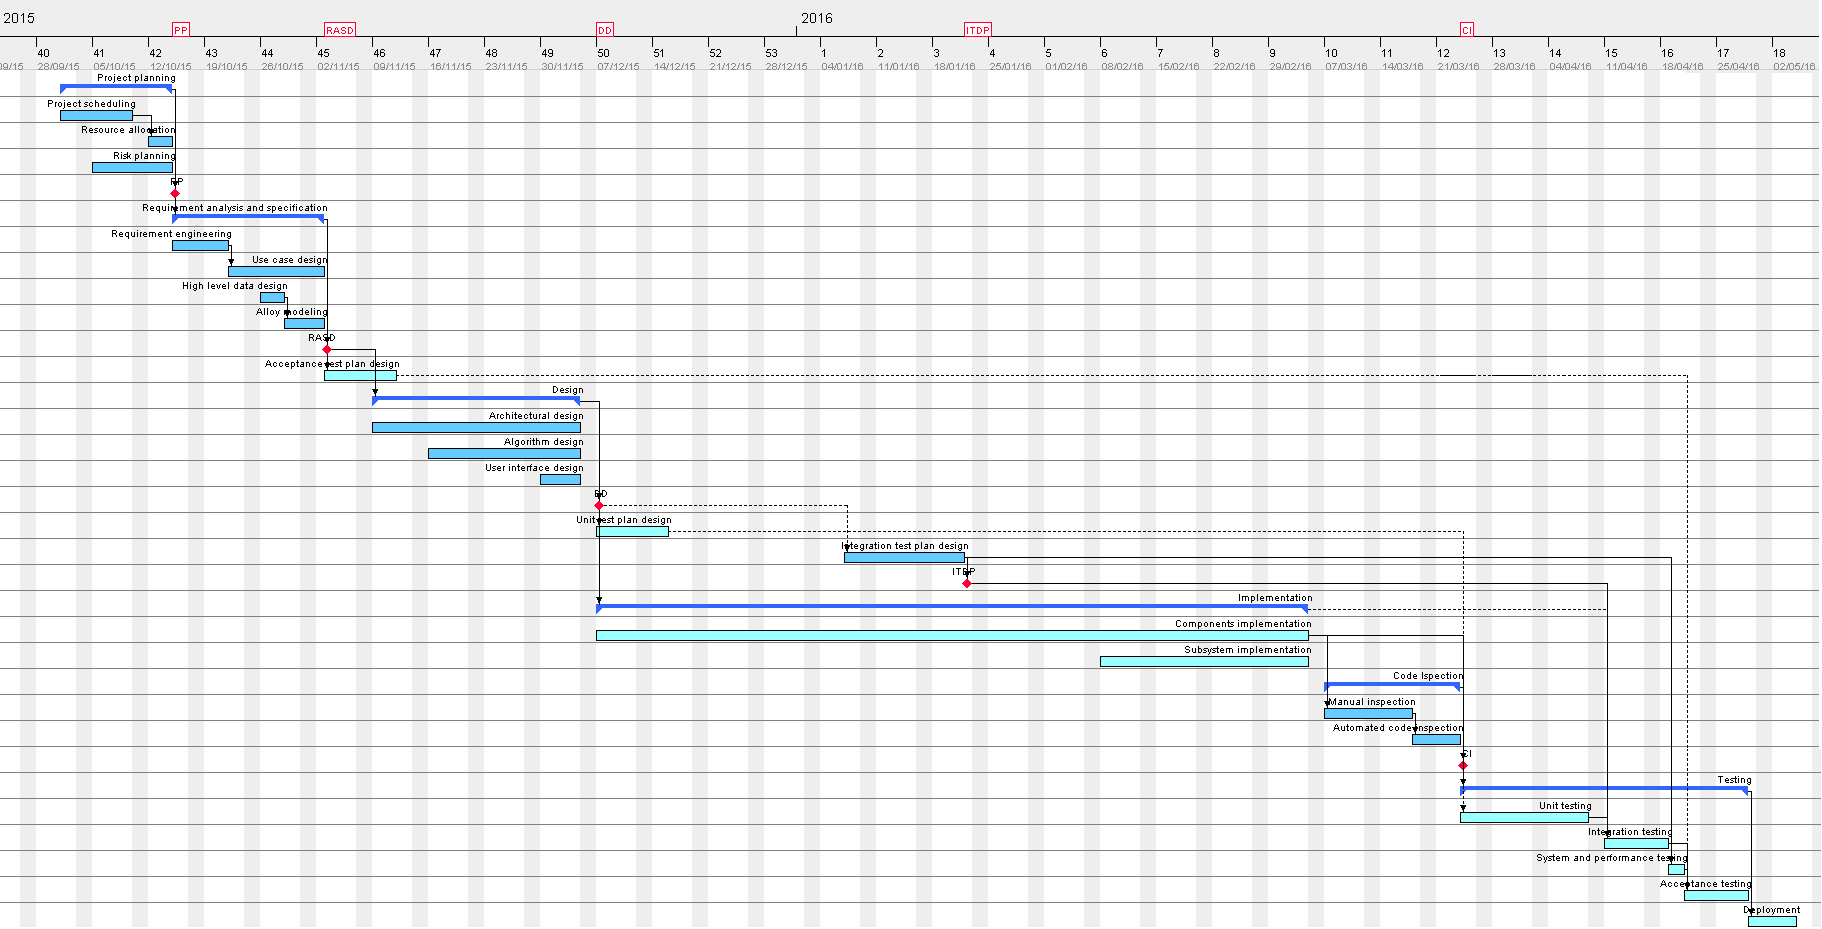
\includegraphics[scale=0.53]{tasks/gantt}

\restoregeometry

\end{landscape}


\clearpage{}


\section{Resources}

In this section we present the \emph{resource allocation}. For each
member of the team we will associate the tasks, as defined in the
previous section, to be executed with reference to the available time
of each team member. Since all team members contributed to the project
playing different roles in the context of the software development
cycle we will specify that role time by time.


\subsection{Resource allocation}

For the task we actually performed the hours specified are the real
ones, for the others we estimated a reasonable allocation of time
also according to our availability being university students. Moreover,
according to our previous experiences, we qualified the implementation
and the testing phases as the most time consuming. 

The following table shows for each task the role played by the team
member and the hours allocated; the attribute ``Units'', as commonly
used in resource planning is the percentage ratio between the used
hours and the allocated hours computed as the duration in days times
8 hours per day. As emerges from the table those values are by far
lower than 50\% because of our university activity.

\begin{landscape}

\begin{tabular}{l|>{\raggedright}p{6.5cm}|>{\centering}m{1.5cm}|>{\centering}p{3.5cm}|c|c|>{\centering}p{3.5cm}|c|c}
\hline 
\multirow{2}{*}{\emph{Task id}} & \multirow{2}{6.5cm}{\emph{Name}} & \multirow{2}{1.5cm}{\emph{Duration}} & \multicolumn{3}{c|}{\textbf{\emph{Riccardo Mologni}}} & \multicolumn{3}{c}{\textbf{\emph{Alberto Maria Metelli}}}\tabularnewline
\cline{4-9} 
 &  &  & \emph{Role} & \textit{Hours} & \emph{Units} & \textit{Role} & \emph{Hours} & \emph{Units}\tabularnewline
\hline 
\hline 
T1 & \textbf{Project planning} & 10 & {\small{}Project Manager} & 10 & 12,5\% & {\small{}Project Manager} & 10 & 12,5\%\tabularnewline
\hline 
T11 & {\footnotesize{}Project scheduling} & 7 & {\small{}Project Manager} & 5 & 8,9\% & {\small{}Project Manager} & 3 & 5,4\%\tabularnewline
\hline 
T12 & {\footnotesize{}Resource allocation} & 3 & {\small{}Project Manager} & 3 & 12,5\% & {\small{}Project Manager} & 3 & 12,5\%\tabularnewline
\hline 
T13 & {\footnotesize{}Risk planning} & 8 & {\small{}Project Manager} & 2 & 3,1\% & {\small{}Project Manager} & 4 & 6,3\%\tabularnewline
\hline 
T2 & \textbf{Requirement analysis and specification} & 13 & {\small{}Analyst} & 33 & 31,7\% & {\small{}Analyst} & 33 & 31,7\%\tabularnewline
\hline 
T21 & {\footnotesize{}Requirement engineering} & 5 & {\small{}Requirements engineer} & 12 & 30,0\% & {\small{}Requirements engineer} & 12 & 30,0\%\tabularnewline
\hline 
T22 & {\footnotesize{}Use case design} & 8 & {\small{}Analyst} & 15 & 23,4\% & {\small{}Analyst} & 11 & 17,2\%\tabularnewline
\hline 
T23 & {\footnotesize{}High level data design} & 3 & {\small{}Analyst} & 3 & 12,5\% & {\small{}Analyst} & 3 & 12,5\%\tabularnewline
\hline 
T24 & {\footnotesize{}Alloy modeling} & 3 & {\small{}Analyst} & 3 & 12,5\% & {\small{}Analyst} & 7 & 29,2\%\tabularnewline
\hline 
T3 & \textbf{Acceptance test plan design} & 7 & {\small{}Analyst} & 8 & 14,3\% & {\small{}Analyst} & 8 & 14,3\%\tabularnewline
\hline 
T4 & \textbf{Design} & 20 & {\small{}Software Architect} & 30 & 18,8\% & {\small{}Software Architect} & 35 & 21,9\%\tabularnewline
\hline 
T41 & {\footnotesize{}Architectural design} & 20 & {\small{}Software Architect} & 15 & 9,4\% & {\small{}Software Architect} & 15 & 9,4\%\tabularnewline
\hline 
T42 & {\footnotesize{}Algorithm design} & 15 & {\small{}Software Architect} & 7 & 5,8\% & {\small{}Software Architect} & 15 & 12,5\%\tabularnewline
\hline 
T43 & {\footnotesize{}User interface design} & 5 & {\small{}Software Architect} & 8 & 20,0\% & {\small{}Software Architect} & 5 & 12,5\%\tabularnewline
\hline 
T5 & \textbf{Unit test plan design} & 7 & {\small{}Analyst} & 13 & 23,2\% & {\small{}Analyst} & 13 & 23,2\%\tabularnewline
\hline 
T6 & \textbf{Integration test plan design} & 11 & {\small{}Analyst} & 12 & 13,6\% & {\small{}Analyst} & 12 & 13,6\%\tabularnewline
\hline 
T7 & \textbf{Implementation} & 65 & {\small{}Developer} & 260 & 50,0\% & {\small{}Developer} & 260 & 50,0\%\tabularnewline
\hline 
T71 & {\footnotesize{}Components implementation} & 65 & {\small{}Developer} & 200 & 38,5\% & {\small{}Developer} & 200 & 38,5\%\tabularnewline
\hline 
T72 & {\footnotesize{}Subsystem implementation} & 20 & {\small{}Developer} & 60 & 37,5\% & {\small{}Developer} & 60 & 37,5\%\tabularnewline
\hline 
T8 & \textbf{Code Ispection} & 13 & {\small{}Ispector} & 15 & 14,4\% & {\small{}Ispector} & 18 & 17,3\%\tabularnewline
\hline 
T81 & {\footnotesize{}Manual inspection} & 9 & {\small{}Ispector} & 13 & 18,1\% & {\small{}Ispector} & 13 & 18,1\%\tabularnewline
\hline 
T82 & {\footnotesize{}Automated code inspection} & 4 & {\small{}Ispector} & 2 & 6,3\% & {\small{}Ispector} & 5 & 15,6\%\tabularnewline
\hline 
T9 & \textbf{Testing} & 26 & {\small{}Tester} & 86 & 41,3\% & {\small{}Tester} & 86 & 41,3\%\tabularnewline
\hline 
T91 & {\footnotesize{}Unit testing} & 12 & {\small{}Tester} & 45 & 46,9\% & {\small{}Tester} & 45 & 46,9\%\tabularnewline
\hline 
T92 & {\footnotesize{}Integration testing} & 6 & {\small{}Tester} & 25 & 52,1\% & {\small{}Tester} & 25 & 52,1\%\tabularnewline
\hline 
T93 & {\footnotesize{}System and performance testing} & 2 & {\small{}Tester} & 6 & 37,5\% & {\small{}Tester} & 6 & 37,5\%\tabularnewline
\hline 
T94 & {\footnotesize{}Acceptance testing} & 6 & {\small{}Tester} & 10 & 20,8\% & {\small{}Tester} & 10 & 20,8\%\tabularnewline
\hline 
T10 & \textbf{Deployment} & 4 & {\small{}Installer} & 15 & 46,9\% & {\small{}Installer} & 15 & 46,9\%\tabularnewline
\hline 
\end{tabular}

\end{landscape}

\begin{landscape}

The following is the same table in which just macro tasks are represented.

\medskip{}


\begin{tabular}{l|>{\raggedright}p{6.5cm}|>{\centering}m{1.5cm}|>{\centering}p{3.5cm}|c|c|>{\centering}p{3.5cm}|c|c}
\hline 
\multirow{2}{*}{\emph{Task id}} & \multirow{2}{6.5cm}{\emph{Name}} & \multirow{2}{1.5cm}{\emph{Duration}} & \multicolumn{3}{c|}{\textbf{\emph{Riccardo Mologni}}} & \multicolumn{3}{c}{\textbf{\emph{Alberto Maria Metelli}}}\tabularnewline
\cline{4-9} 
 &  &  & \emph{Role} & \textit{Hours} & \emph{Units} & \textit{Role} & \emph{Hours} & \emph{Units}\tabularnewline
\hline 
\hline 
T1 & Project planning & 10 & {\small{}Project Manager} & 10 & 12,5\% & {\small{}Project Manager} & 10 & 12,5\%\tabularnewline
\hline 
T2 & Requirement analysis and specification & 13 & {\small{}Analyst} & 33 & 31,7\% & {\small{}Analyst} & 33 & 31,7\%\tabularnewline
\hline 
T3 & Acceptance test plan design & 7 & {\small{}Analyst} & 8 & 14,3\% & {\small{}Analyst} & 8 & 14,3\%\tabularnewline
\hline 
T4 & Design & 20 & {\small{}Software Architect} & 30 & 18,8\% & {\small{}Software Architect} & 35 & 21,9\%\tabularnewline
\hline 
T5 & Unit test plan design & 7 & {\small{}Analyst} & 13 & 23,2\% & {\small{}Analyst} & 13 & 23,2\%\tabularnewline
\hline 
T6 & Integration test plan design & 11 & {\small{}Analyst} & 12 & 13,6\% & {\small{}Analyst} & 12 & 13,6\%\tabularnewline
\hline 
T7 & Implementation & 65 & {\small{}Developer} & 260 & 50,0\% & {\small{}Developer} & 260 & 50,0\%\tabularnewline
\hline 
T8 & Code Ispection & 13 & {\small{}Ispector} & 15 & 14,4\% & {\small{}Ispector} & 18 & 17,3\%\tabularnewline
\hline 
T9 & Testing & 26 & {\small{}Tester} & 86 & 41,3\% & {\small{}Tester} & 86 & 41,3\%\tabularnewline
\hline 
T10 & Deployment & 4 & {\small{}Installer} & 15 & 46,9\% & {\small{}Installer} & 15 & 46,9\%\tabularnewline
\hline 
\end{tabular}

\end{landscape}


\subsection{Cumulative data}

In this subsection we report some cumulative data derived from the
previous table. We want to make a clear distinction between real deta
referred to the task we actually performed and estimated data.


\subsubsection{Estimated data}
\begin{itemize}
\item \emph{Total duration}: 176 days (1408 h)
\item \emph{Total working hours}

\begin{itemize}
\item Riccardo Mologni: 482 h
\item Alberto Maria Metelli: 490 h
\end{itemize}
\item \emph{Working hours per day}

\begin{itemize}
\item Riccardo Mologni: 2,72 h/day
\item Alberto Maria Metelli: 2,78 h/day
\end{itemize}
\item \emph{Units}

\begin{itemize}
\item Riccardo Mologni: 34,2\%
\item Alberto Maria Metelli: 34,8\%
\end{itemize}
\end{itemize}

\subsubsection{Real data}
\begin{itemize}
\item \emph{Total duration}: 67 days (536 h)
\item \emph{Total working hours}

\begin{itemize}
\item Riccardo Mologni: 100 h
\item Alberto Maria Metelli: 108 h
\end{itemize}
\item \emph{Working hours per day}

\begin{itemize}
\item Riccardo Mologni: 0,57 h/day
\item Alberto Maria Metelli: 0,61 h/day
\end{itemize}
\item \emph{Units}

\begin{itemize}
\item Riccardo Mologni: 18,7\%
\item Alberto Maria Metelli: 20,1\%
\end{itemize}
\end{itemize}
\begin{landscape}

\newgeometry{left=2.5cm,bottom=0cm,top=2.5cm,right=-7cm}


\subsection{Resource allocation chart}

\medskip{}


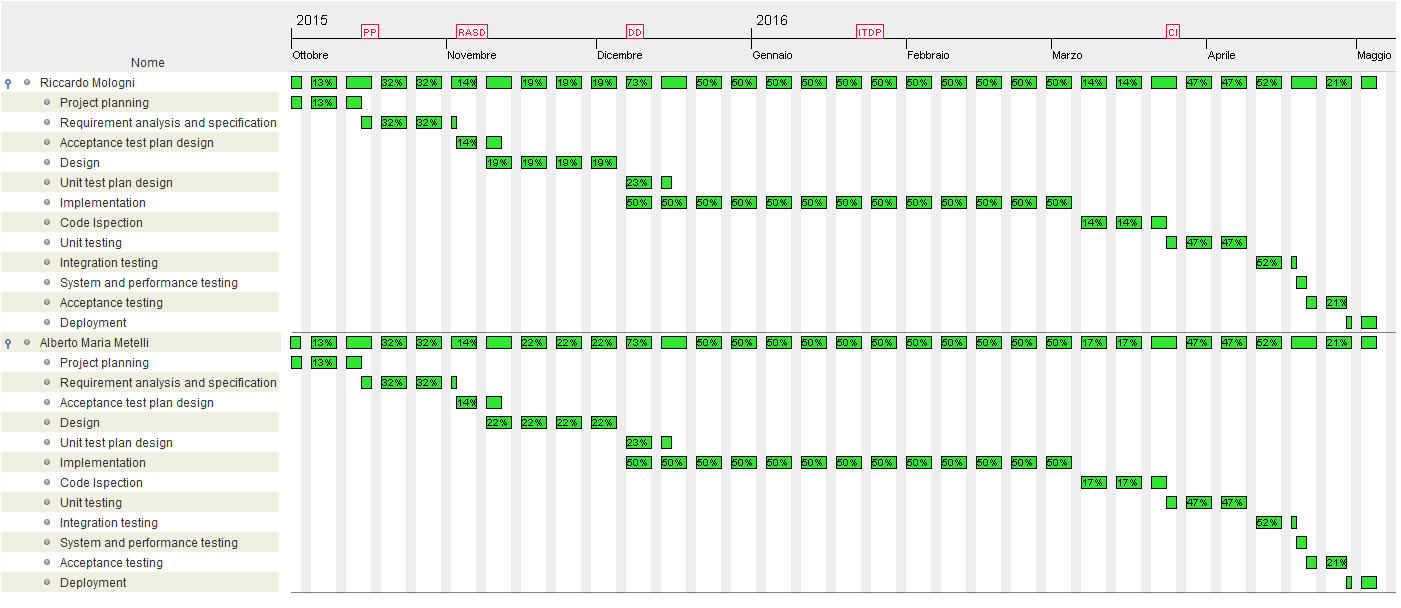
\includegraphics[scale=0.7]{resources/resources}

\restoregeometry

\end{landscape}


\clearpage{}


\section{Risks and recovery actions}

A \emph{risk }is a potential condition that can lead to a the loss
of some value, either resource (economic or not) or time. \emph{Risk
Mitigation, Monitoring, and Management} (\emph{RMMM}) is a key step
of any project plan, it is intended to help to pre-determine any possible
major risks that may occur during development of this software. In
this section we will identify the main risks concerning the development
of myTaxiService and we will propose some strategy to tackle them.


\subsection{Introduction}

In this section we provide an analysis of the main risks harming the
myTaxiService project. For each risk identified we will provide the
the corresponding category \emph{project risks},\emph{ technical risks
}and\emph{ business risks, }an estimation of the probability and the
impact on the project %
\footnote{Probability and impact are expressed according to the standard qualitative
scale. For probability: Certain, Likely, Possible, Unlikely, Rare.
For impact/effect: Negligible, Marginal, Critical, Catastrophic.%
}.


\subsubsection{Project risks}

\emph{Project risks} (also known as development risks) are risks that
might threaten the project plan, if one of them becomes real it will
harm the project schedule, making it slip and increase the overall
cost. In myTaxiService we identified the following project risks.

\medskip{}


\begin{tabular}{>{\raggedright}p{4cm}|>{\raggedright}p{5cm}|>{\centering}p{2cm}|>{\centering}p{2cm}}
\hline 
\emph{Name} & \emph{Description} & \emph{Probability} & \emph{Impact}\tabularnewline
\hline 
\hline 
\emph{Requirement problem - 1} & Requirement engineers misunderstood the the requirements. & Possible & Catastrophic\tabularnewline
\hline 
\emph{Requirement problem - 2} & Customers changes the requirement in the late phases of the software
development. & Possible & Catastrophic\tabularnewline
\hline 
\emph{Requirement problem - 3} & The customer is not available when needed & Likely & Marginal\tabularnewline
\hline 
\emph{Personnel problem - 1} & Project manager is absent at critical times in the project. & Unlikely & Critical\tabularnewline
\hline 
\emph{Personnel problem - 2} & Some team members are absent at the critical times in the project. & Unlikely & Marginal\tabularnewline
\hline 
\emph{Personnel problem - 3} & Development team is not qulified to program a complex application
with JEE. & Likely & Critical\tabularnewline
\hline 
\emph{Personnel problem - 4} & Miscommunication in the project team. & Possible & Critical\tabularnewline
\hline 
\emph{Personnel problem - 5} & Lack of documentation. & Rare & Critical\tabularnewline
\hline 
\end{tabular}


\subsubsection{Business risks}

\emph{Business risks} can threaten the viability of the software to
be produced; if one of them becomes real it can compromise the economic
success of the project. In myTaxiService system we identified the
following business risks.

\medskip{}


\begin{tabular}{>{\raggedright}p{4cm}|>{\raggedright}p{5cm}|>{\centering}p{2cm}|>{\centering}p{2cm}}
\hline 
\emph{Name} & \emph{Description} & \emph{Probability} & \emph{Impact}\tabularnewline
\hline 
\hline 
\emph{Market risk} & There is no demand for product, passengers prefer to use the traditional
channels to call for a taxi. & Possible & Catastrophic\tabularnewline
\hline 
\emph{Budget risk} & Due to organizational financial problems the budget is reduced. & Unlikely & Catastrophic\tabularnewline
\hline 
\end{tabular}


\subsubsection{Technical risks}

\emph{Technical risks} can threaten the quality and the timeliness
of the software to be developed; if a technical risk becomes real
it can make the implementation more difficult or even impossible.
In myTaxiService system we identified the following technical risks.

\medskip{}


\begin{tabular}{>{\raggedright}p{4cm}|>{\raggedright}p{5cm}|>{\centering}p{2cm}|>{\centering}p{2cm}}
\hline 
\emph{Name} & \emph{Description} & \emph{Probability} & \emph{Impact}\tabularnewline
\hline 
\hline 
\emph{Design problem - 1} & The architectural style and patter chosen in the architectural design
phase are not suitable for the kind of application to be developed. & Unlikely & Catastrophic\tabularnewline
\hline 
\emph{Design problem - 2} & The algorithm for taxi management proposed in the design phase are
not correct.  & Rare & Serious\tabularnewline
\hline 
\emph{Design problem - 3} & Design does not reflect requirements & Unlikely & Catastrophic\tabularnewline
\hline 
\emph{Implementation problem - 1} & Poor comments in the code. & Possible & Marginal\tabularnewline
\hline 
\emph{Implementation problems - 2} & Code does not follow quality guidelines. & Unlikely & Critical\tabularnewline
\hline 
\emph{Implementation problem - 3} & The code does not reflect the designed architecture. & Unlikely & Critical\tabularnewline
\hline 
\emph{Performance problems - 1} & The DBMS cannot meet the performance requirements.  & Unlikely & Catastrophic\tabularnewline
\hline 
\end{tabular}


\subsection{Risk strategy}

A \emph{risk strategy} defines a set of rules to be applied in order
to manage and tackle risk. Those strategies are typically divided
into:
\begin{itemize}
\item \emph{Reactive risk strategies}: there is no explicit risk management,
nothing is done about risk until something goes wrong. This is the
typical approach that is adopted by the majority of software teams
and managers. This strategy is also known as \emph{crisis management}
since no preventive measure is designed.
\item \emph{Proactive risk strategies}: risk identification, analysis and
ranking are performed in advance in order to develop a \emph{contingency}
plan to manage risk having high probability and high impact. This
approach, even if more costly, is aimed to avoid risk in order to
be able to deal with only unforeseen risks.
\end{itemize}
Since in the previous section we have identified the risks, we are
actually following the proactive risk strategy. We think that identifying
the risks, set up proper measures in order to tackle them in an appropriate
way would make smaller the economic effort in the future stages.

\begin{figure}[H]
\noindent \begin{centering}
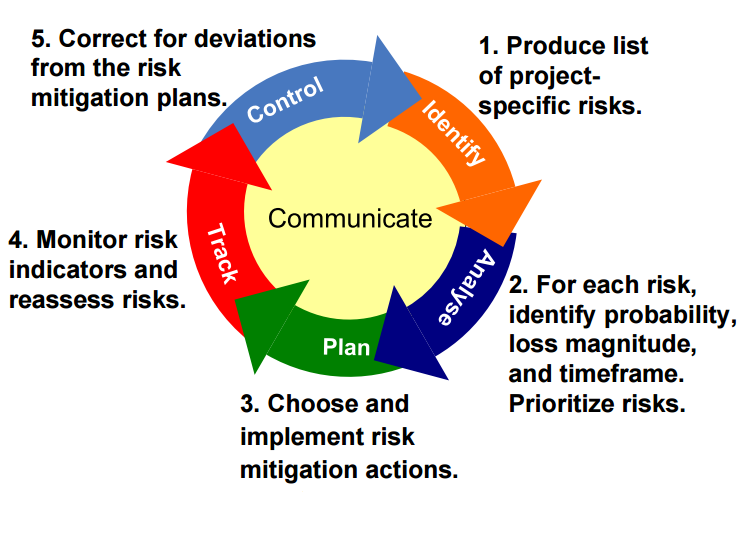
\includegraphics[scale=0.75]{risks/images/risk}
\par\end{centering}

\protect\caption{Proactive risk strategy cycle}
\end{figure}


In the following tables we report for each risk identified in the
previous section a possible \emph{prevention plan} or a \emph{correction
plan}.

\begin{landscape}


\subsubsection{Project risks}

\medskip{}


\begin{tabular}{>{\raggedright}p{4cm}|>{\raggedright}p{10cm}|>{\raggedright}p{8cm}}
\hline 
\emph{Name} & \emph{Prevention} & \emph{Correction}\tabularnewline
\hline 
\hline 
\emph{Requirement problem - 1} & \begin{itemize}
\item {\small{}Adopt a formalized method for requirement engineering (like
Jackson-Zave approach).}{\small \par}
\item {\small{}Perform validation of requirements right before design phase
by meeting the stakeholders.}{\small \par}
\item {\small{}After requirement engineering phase provide customers with
a small prototype.}\end{itemize}
 & {\small{}Recycle on the requirement engineering phase fixing the RASD.}\tabularnewline
\hline 
\emph{Requirement problem - 2} & \begin{itemize}
\item {\small{}It is explained to the customer, that after he has accepted
a version of the RASD, it cannot be changed by the customer’s wish
only.}{\small \par}
\item {\small{}Trace the requirements in order to quantify the effort of
changing.}\end{itemize}
 & {\small{}Recycle on the requirement engineering phase fixing the RASD.}\tabularnewline
\hline 
\emph{Requirement problem - 3} & \begin{itemize}
\item {\small{}Try to stay in touch with the customer in order to increase
his interest on the product.}{\small \par}
\item {\small{}Meetings with the customer can be planned well in advance.}\end{itemize}
 & {\small{}When the customer is not available, meetings may have to
be rescheduled. }\tabularnewline
\hline 
\emph{Personnel problem - 1} & {\small{}Nominate a vice project manager.} & {\small{}Vice project manager takes over the role of the project manager.}\tabularnewline
\hline 
\emph{Personnel problem - 2} & \begin{itemize}
\item {\small{}Team members should warn the project manager timely before
a planned period of absence.}{\small \par}
\item {\small{}Ensure that knowledge is shared between team members}\end{itemize}
 & {\small{}An other team member takes care of the work.}\tabularnewline
\hline 
\end{tabular}

\begin{tabular}{>{\raggedright}p{4cm}|>{\raggedright}p{10cm}|>{\raggedright}p{8cm}}
\hline 
\emph{Name} & \emph{Prevention} & \emph{Correction}\tabularnewline
\hline 
\hline 
\emph{Personnel problem - 3} & {\small{}Provide an introductory course to JEE} & \tabularnewline
\hline 
\emph{Personnel problem - 4} & \begin{itemize}
\item {\small{}After a meeting, one group member creates an interview report. }{\small \par}
\item {\small{}Team members should not hesitate to ask and re-ask questions
if things are unclear.}\end{itemize}
 & {\small{}When it becomes clear that miscommunication is causing problems,
the team members involved and the customer are gathered in a meeting
to clear things up.}\tabularnewline
\hline 
\emph{Personnel problem - 5} & {\small{}Impose that before starting a new phase of the software development
the corresponding document is ready.} & {\small{}Ask the employee to write documentation.}\tabularnewline
\hline 
\end{tabular}

\medskip{}



\subsubsection{Business risks}

\medskip{}


\begin{tabular}{>{\raggedright}p{4cm}|>{\raggedright}p{10cm}|>{\raggedright}p{8cm}}
\hline 
\emph{Name} & \emph{Prevention} & \emph{Correction}\tabularnewline
\hline 
\hline 
\emph{Market risk} & {\small{}Make sure there is the interest around the product.} & {\small{}Advertise the product.}\tabularnewline
\hline 
\emph{Budget risk} & {\small{}Make sure at the beginning of the project that there is the
availability of budget.} & {\small{}Communicate with the founders showing how the project makes
a contribution to the goals of the business and argument about the
fact that cuts to the budget would not be cost effective.}\tabularnewline
\hline 
\end{tabular}

\newpage{}


\subsubsection{Technical risks}

\medskip{}


\begin{tabular}{>{\raggedright}p{4cm}|>{\raggedright}p{10cm}|>{\raggedright}p{8cm}}
\hline 
\emph{Name} & \emph{Prevention} & \emph{Correction}\tabularnewline
\hline 
\hline 
\emph{Design problem - 1} & \begin{itemize}
\item {\small{}Perform inspection of the DD.}{\small \par}
\item {\small{}Ask some advisor on his opinion about the feasibility and
the correctness of certain design decisions.}\end{itemize}
 & \begin{itemize}
\item {\small{}When errors in the design are noticed consulted some advisor
to help correct the design errors as soon as possible. }{\small \par}
\item {\small{}Also all the work, that depends on the faulty design, should
be halted until the error is corrected.}\end{itemize}
\tabularnewline
\hline 
\emph{Design problem - 2} & {\small{}Use simulation techniques to test the correctness of the
algorithm} & {\small{}Revise the algorithm in order to fix the flaws.}\tabularnewline
\hline 
\emph{Design problem - 3} & \begin{itemize}
\item {\small{}Perform inspection of the DD.}{\small \par}
\item {\small{}Show at least some part of the DD to the customer in order
to see his/her opinion.}\end{itemize}
 & {\small{}Recycle on the design phase fixing the DD.}\tabularnewline
\hline 
\emph{Implementation problem - 1} & {\small{}Provide the developer with a clear specification of what
to comment.} & {\small{}Ask the developer to add the missing comments.}\tabularnewline
\hline 
\emph{Implementation problems - 2} & \begin{itemize}
\item {\small{}Provide the developer with a document in which code conventions
are stated.}{\small \par}
\item {\small{}Perform code inspection.}\end{itemize}
 & {\small{}Ask the developer to fix the issues.}\tabularnewline
\hline 
\emph{Implementation problem - 3} & \begin{itemize}
\item {\small{}Perform unit testing after each module is ready}{\small \par}
\item {\small{}Continuesly check the work of the developers}\end{itemize}
 & {\small{}Ask the developer to fix the involved component.}\tabularnewline
\hline 
\emph{Performance problems - 1} & {\small{}Estimate the load and acquire a suitable DBMS.} & {\small{}Investigate the possibility of acquiring a highier performance
DBMS.}\tabularnewline
\hline 
\end{tabular}

\end{landscape}


\clearpage{}

\appendix

\thispagestyle{empty}

\section{Appendix} \label{sec:Appendix1}


\subsection*{Used tools}
\begin{enumerate}
\item \LyX{} visual editor for \LaTeX{} (\url{http://www.lyx.org/}) to
write this document.
\item GanttProject for the Gantt diagram and the resource diagram \url{http://www.ganttproject.biz/}. 
\end{enumerate}

\subsection*{Hours of works}

Time spent by each group member:
\begin{itemize}
\item Alberto Maria Metelli: 10 h
\item Riccardo Mologni: 10 h
\end{itemize}

\subsection*{Revision history}
\begin{lyxlist}{00.00.0000}
\item [{%
\begin{tabular}{>{\raggedright}p{1.5cm}|>{\raggedright}p{2cm}|>{\raggedright}p{3.5cm}|>{\raggedright}p{5cm}}
\hline 
\emph{Version} & \emph{Date} & \emph{Revision description} & \emph{Revision notes}\tabularnewline
\hline 
0.1 &  & Initial draft & -\tabularnewline
\hline 
1.0 & 2-2-2016 & Final draft & -\tabularnewline
\hline 
\end{tabular}}]~\end{lyxlist}




\section*{\clearpage{}}
\end{document}
